\documentclass[12pt]{amsart}
\usepackage{amsthm,amssymb,amsmath}
\usepackage{graphicx}
\usepackage{subcaption}   % side-by-side sub-figures (modern replacement for subfigure)
\usepackage{natbib}
\usepackage{dsfont}
\usepackage{multirow}
\usepackage{booktabs}     % \toprule, \midrule, \bottomrule for clean tables
\usepackage{float}
\usepackage{listings}     % Python code in the appendix

% ---- page layout (from the course template) ----
\textwidth 175mm
\oddsidemargin -5mm
\evensidemargin -5mm
\textheight 230mm
\topmargin -10mm

% ---- helpers ----
% \TODO{...} prints a bold reminder in the PDF. Search for "TODO" before submitting: none should be left.
\newcommand{\TODO}[1]{\textbf{[TODO: #1]}}
\newcommand{\Q}{\mathbb{Q}}
\newcommand{\PP}{\mathbb{P}}
\newcommand{\N}{\mathcal{N}}

\lstset{language=Python, basicstyle=\ttfamily\footnotesize, breaklines=true,
        frame=single, numbers=left, numberstyle=\tiny, showstringspaces=false}

\title[Discrete- vs.\ Continuous-Time Models]{STA2503 Project 1: Discrete-Time vs.\ Continuous-Time Financial Models}
\author{Alec Neme}
% \email{...}   % TODO: add your UofT email if the course wants it

\begin{document}

\begin{abstract}
\TODO{Write this LAST, in two short paragraphs. (1) What you did: simulated scaled random walks
and Brownian motion; priced a 1-year at-the-money European call on NVIDIA with a CRR binomial tree
and with Monte Carlo under GBM; compared both with Black--Scholes. (2) Main findings, with the
actual numbers: e.g.\ ``the binomial price converges to the Black--Scholes value of \$X as $N$
grows; the Monte Carlo estimate is \$Y $\pm$ Z''.}
\end{abstract}

\maketitle

% =====================================================================
\section{Introduction}
% =====================================================================
\TODO{3--5 sentences. Why compare discrete- and continuous-time models? (The binomial model is
intuitive and exact under no-arbitrage for finite $N$; Black--Scholes/GBM is the continuous-time
limit.) State the plan of the report (Part I: random walk $\to$ Brownian motion; Part II: CRR
vs.\ GBM for NVDA) and the headline result in one sentence.}

% =====================================================================
\section{Methodology}
% =====================================================================

\subsection{Brownian motion and scaled random walks}
Let $(\Omega,\mathcal F,\{\mathcal F_t\}_{t\ge 0},\PP)$ be a filtered probability space.
A process $W=\{W_t\}_{t\ge0}$ is a \emph{standard Brownian motion} if
\begin{enumerate}
  \item $W_0=0$ and $W$ is adapted to $\{\mathcal F_t\}$;
  \item for $0\le s\le t$, $W_t-W_s\sim\N(0,\,t-s)$;
  \item $W_t-W_s$ is independent of $\mathcal F_s$;
  \item $t\mapsto W_t(\omega)$ is continuous for every $\omega\in\Omega$.
\end{enumerate}

\noindent\textbf{Simulating BM.} On the grid $t_k=k\Delta t$, $\Delta t=1/N_1$, we use
\begin{equation}\label{eq:bm_scheme}
W_{t_{k+1}} = W_{t_k} + \sqrt{\Delta t}\,\xi_{k+1},\qquad \xi_k \overset{iid}{\sim}\N(0,1),\qquad W_0=0,
\end{equation}
which is exact at the grid points by property 2. We take $N_1=10{,}000$.

\noindent\textbf{Scaled random walk.} Let $Z_i\overset{iid}{\sim}\pm1$ with probability $\tfrac12$ each, and
\begin{equation}\label{eq:srw}
W^{(N)}_t = \frac{1}{\sqrt N}\sum_{i=1}^{Nt} Z_i,\qquad t\in\{0,\tfrac1N,\dots,1\}.
\end{equation}
Each increment of $W^{(N)}$ has mean $0$ and variance $1/N=\Delta t$, matching those of BM.
We simulate $N_2\in\{10,50,200,1000\}$.
\TODO{Optional 1--2 sentences: why the $1/\sqrt N$ scaling (it is the only scaling that keeps
$\operatorname{Var}(W^{(N)}_1)=1$ as $N\to\infty$).}

\subsection{The CRR binomial model}
With $N$ steps over $[0,T]$ and $\Delta t = T/N$, the stock moves from $S$ to $uS$ or $dS$, where
\begin{equation}\label{eq:crr}
u=e^{\sigma\sqrt{\Delta t}},\qquad d=\frac1u,\qquad \tilde p=\frac{e^{r\Delta t}-d}{u-d}.
\end{equation}
No arbitrage requires $d<e^{r\Delta t}<u$, which holds for our parameters.
\TODO{1 sentence: note that $e^{r\Delta t}$ is the continuously-compounded version of the $1+r$
used in lecture.}
After $n$ steps with $j$ up-moves the price is $S_n(j)=S_0\,u^{j}d^{\,n-j}$, $j=0,\dots,n$.
A European call is priced by backward induction:
\begin{equation}\label{eq:backward}
V_N(j)=\bigl(S_N(j)-K\bigr)^+,\qquad
V_n(j)=e^{-r\Delta t}\Bigl[\tilde p\,V_{n+1}(j+1)+(1-\tilde p)\,V_{n+1}(j)\Bigr],
\end{equation}
and the price is $V_0(0)$.
\TODO{Figure of the tree (small $N$, e.g.\ 3 or 4) with prices at the nodes -- produced in Notebook 02.}

\subsection{Geometric Brownian motion}
Under GBM, $dS_t=\mu S_t\,dt+\sigma S_t\,dW_t$. Applying It\^o's formula to $\log S_t$,
\[
d\log S_t=\Bigl(\mu-\tfrac12\sigma^2\Bigr)dt+\sigma\,dW_t
\quad\Longrightarrow\quad
S_t=S_0\exp\Bigl[\Bigl(\mu-\tfrac12\sigma^2\Bigr)t+\sigma W_t\Bigr].
\]
\TODO{Optional: show the It\^o step in one more line ($f(x)=\log x$, $f'=1/x$, $f''=-1/x^2$, $d[S]_t=\sigma^2S_t^2dt$).}

For pricing we work under the risk-neutral measure $\Q$, where $\mu$ is replaced by $r$.
The Euler--Maruyama scheme on the grid $t_k=k\Delta t$ is
\begin{equation}\label{eq:euler}
S_{t_{k+1}} = S_{t_k}\bigl(1+r\Delta t+\sigma\sqrt{\Delta t}\,\xi_{k+1}\bigr),\qquad \xi_k\overset{iid}{\sim}\N(0,1).
\end{equation}
With $M$ simulated paths, the Monte Carlo price and its standard error are
\begin{equation}\label{eq:mc}
\widehat C = e^{-rT}\frac1M\sum_{m=1}^M \bigl(S_T^{(m)}-K\bigr)^+,\qquad
\mathrm{SE}=\frac{s}{\sqrt M},
\end{equation}
where $s$ is the sample standard deviation of the discounted payoffs; a 95\% confidence interval is $\widehat C\pm1.96\,\mathrm{SE}$.

\subsection{Black--Scholes benchmark}
\begin{equation}\label{eq:bs}
C_{BS}=S_0\,\Phi(d_1)-Ke^{-rT}\Phi(d_2),\qquad
d_1=\frac{\ln(S_0/K)+(r+\tfrac12\sigma^2)T}{\sigma\sqrt T},\qquad d_2=d_1-\sigma\sqrt T.
\end{equation}

\subsection{Assumptions}
\begin{table}[H]
\centering
\begin{tabular}{lll}
\toprule
Parameter & Value & Source / justification \\
\midrule
$S_0$ & \TODO{\$xxx.xx} & NVDA close on \TODO{date}, from \TODO{website} \\
$K$ & $S_0$ & at-the-money, as required \\
$T$ & 1 year & as required \\
$r$ & 4\% (cont.\ comp.) & suggested in the project \\
$\sigma$ & 30\% annualised & suggested in the project \\
$N$ (tree steps) & \TODO{e.g.\ 50, 100, \dots} & convergence study \\
$M$ (MC paths) & \TODO{e.g.\ 100{,}000} & \\
\bottomrule
\end{tabular}
\caption{Model inputs. \label{tbl:assumptions}}
\end{table}
\TODO{1 sentence: tasks 2(c) and 3 of the project mention Amazon; we treat this as a typo and use NVDA throughout.}

% =====================================================================
\section{Results}
% =====================================================================

\subsection{Scaled random walks and Brownian motion}

\begin{figure}[H]
\centering
\begin{subfigure}{0.49\textwidth}
  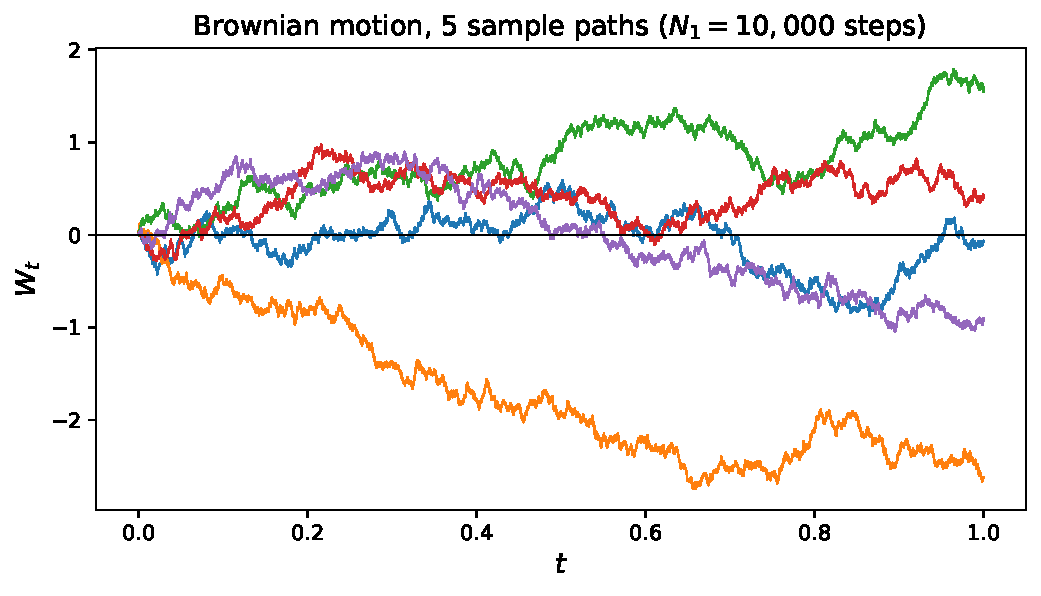
\includegraphics[width=\linewidth]{figures/part1_bm_paths.pdf}
  \caption{Brownian motion, $N_1=10{,}000$.}
\end{subfigure}\hfill
\begin{subfigure}{0.49\textwidth}
  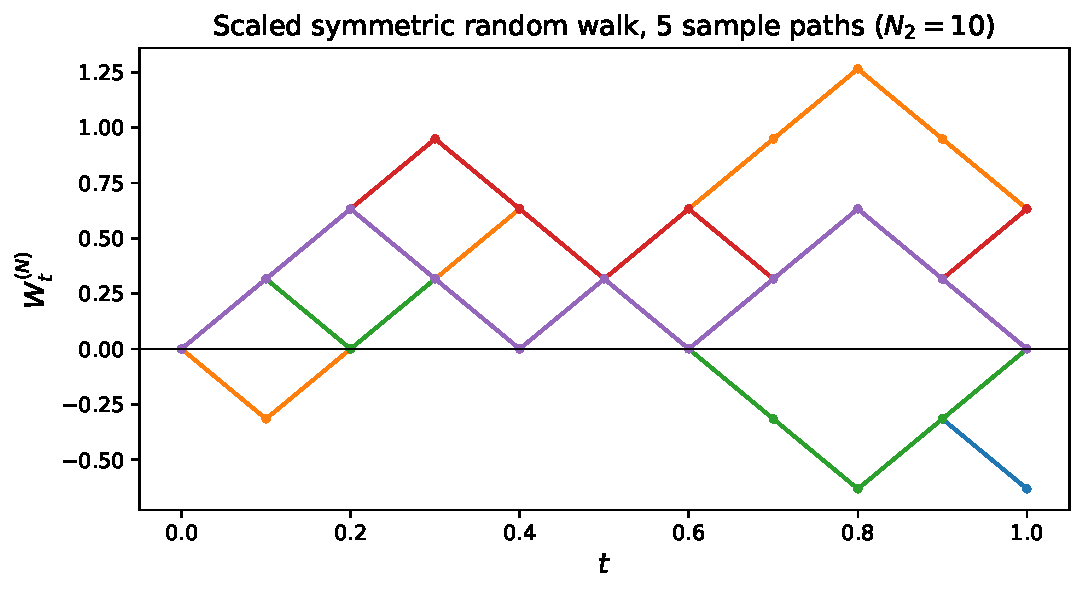
\includegraphics[width=\linewidth]{figures/part1_rw_N10.pdf}
  \caption{Scaled random walk, $N_2=10$.}
\end{subfigure}
\caption{Five sample paths of each process on $[0,1]$. \label{fig:bm_rw10}}
\end{figure}

\begin{figure}[H]
\centering
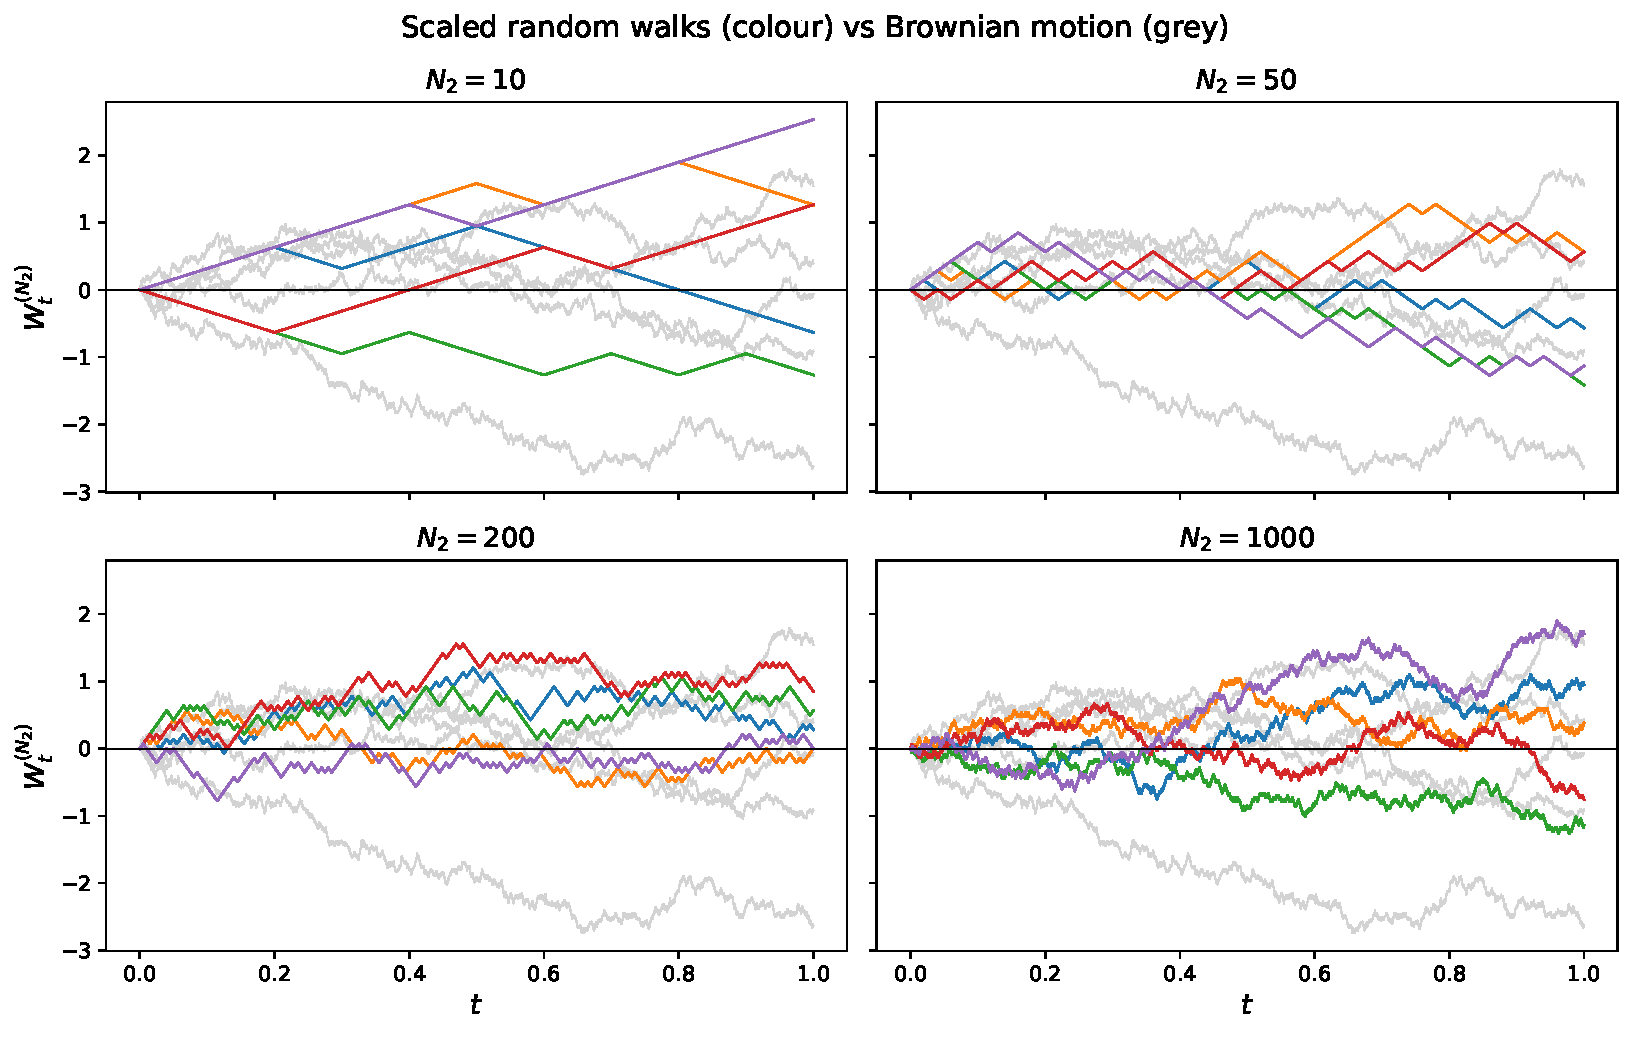
\includegraphics[width=0.9\textwidth]{figures/part1_rw_vs_bm.pdf}
\caption{Scaled random walks (colour) for increasing $N_2$, with the Brownian motion paths of
Figure~\ref{fig:bm_rw10}(a) in grey. \label{fig:rw_vs_bm}}
\end{figure}

\noindent\textbf{Discussion.}

As we can see from Figure~\ref{fig:rw_vs_bm}, for small $N_2$ the simulated random walks are
piecewise linear: with $N_2 = 10$, each path changes direction only at the grid points
$t = 0.1, 0.2, \dots, 1$ and moves in straight lines in between. The Brownian motion paths
generated with $N_1 = 10{,}000$ steps (in grey), on the other hand, oscillate at every time
scale and show no visible straight segments. When $N_2 = 200$, the scaled random walk starts
looking more like Brownian motion, and for $N_2 = 1000$ the two are indistinguishable in
character, even though the coloured and grey paths are independent realizations.

This happens because Brownian motion is the limit in distribution of the scaled random walk
(Donsker's theorem). As we increase $N_2$, the walk changes value more frequently (every
$1/N_2$ units of time), and at the same time each step shrinks to $\pm 1/\sqrt{N_2}$. The
scaling is done because without it, $\operatorname{Var}(W_1)$ would equal $N_2$ and the walk
would blow up, whereas with it $\operatorname{Var}(W^{(N_2)}_1) = 1$ for every $N_2$. Each
straight segment has slope $\pm\sqrt{N_2}$, which becomes steeper as $N_2$ grows; this is the
discrete counterpart of the fact that Brownian motion paths are not differentiable.

\subsection{Binomial model}
\TODO{Notebook 02: tree figure (small $N$); table/plot of the call price against $N$ with the Black--Scholes value as a horizontal line; 1-year call price for the chosen $N$.}

\subsection{GBM and Monte Carlo}
\TODO{Notebook 03: figure of simulated GBM paths; Monte Carlo price with SE and 95\% CI; (optional) exact vs.\ Euler--Maruyama.}

\subsection{Comparison}
\begin{table}[H]
\centering
\begin{tabular}{lcc}
\toprule
Method & Call price (\$) & Difference from BS (\$) \\
\midrule
CRR binomial, $N=$ \TODO{} & \TODO{} & \TODO{} \\
Monte Carlo (GBM), $M=$ \TODO{} & \TODO{} $\pm$ \TODO{} & \TODO{} \\
Black--Scholes & \TODO{} & -- \\
\bottomrule
\end{tabular}
\caption{One-year at-the-money European call on NVDA. \label{tbl:comparison}}
\end{table}
\TODO{Discussion: is the binomial error shrinking like $1/N$ (with odd/even oscillation)? Is BS inside the MC confidence interval? Trade-offs: speed, accuracy, what each model is good for.}

% =====================================================================
\section{Conclusions}
% =====================================================================
\TODO{3--5 sentences: main findings with numbers, one limitation (e.g.\ constant $\sigma$ and $r$), one possible extension.}

\clearpage
\appendix
\section{Python code}
\TODO{Key functions from the notebooks. Plan: export them to \texttt{project1/code/*.py} and include with
\texttt{\textbackslash lstinputlisting\{../code/part1.py\}}. Check whether the appendix counts toward the 15-page limit.}

\end{document}